\documentclass[tikz,border=2pt]{standalone}
\usetikzlibrary{arrows.meta,positioning,calc,shapes.geometric}
\usepackage{fontspec}
\setmainfont{TeX Gyre Termes}
\setsansfont{Roboto}
\begin{document}
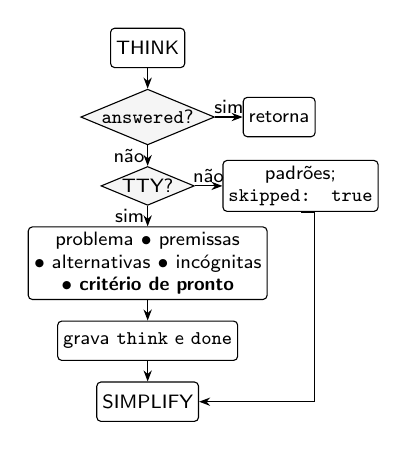
\begin{tikzpicture}[
  font=\sffamily\scriptsize, >={Stealth[length=4pt]},
  proc/.style={draw, thin, rounded corners=1.5pt, align=center, fill=white, minimum height=0.5cm, inner sep=2pt},
  exec/.style={proc, very thick, double distance=0.9pt, fill=black!8},
  dec/.style={draw, thin, diamond, aspect=2.4, align=center, fill=black!4, inner sep=0.5pt, font=\sffamily\scriptsize},
  nota/.style={font=\sffamily\scriptsize, align=center, text=black!80},
  lbl/.style={font=\sffamily\scriptsize, inner sep=1pt}
]
\node[proc] (a) {THINK};
\node[dec, below=0.26cm of a] (g1) {\texttt{answered}?};
\node[proc, right=0.35cm of g1] (r1) {retorna};
\node[dec, below=0.26cm of g1] (g2) {TTY?};
\node[proc, right=0.35cm of g2] (r2) {padrões;\\ \texttt{skipped: true}};
\node[proc, below=0.26cm of g2] (q) {problema $\bullet$ premissas\\
  $\bullet$ alternativas $\bullet$ incógnitas\\
  $\bullet$ \textbf{critério de pronto}};
\node[proc, below=0.26cm of q] (rec) {grava \texttt{think} e \texttt{done}};
\node[proc, below=0.26cm of rec] (n) {SIMPLIFY};
\coordinate (chan) at ($(q.east)+(0.60,0)$);
\draw[->] (a) -- (g1);
\draw[->] (g1) -- node[lbl,above]{sim} (r1);
\draw[->] (g1) -- node[lbl,left]{não} (g2);
\draw[->] (g2) -- node[lbl,above]{não} (r2);
\draw[->] (g2) -- node[lbl,left]{sim} (q);
\draw[->] (q) -- (rec);
\draw[->] (rec) -- (n);
\draw[->] (r2.south) -- (r2.south -| chan) -- (n -| chan) -- (n.east);
\end{tikzpicture}
\end{document}
